\documentclass[11pt]{article}
\usepackage[margin=1in]{geometry}
\usepackage{amssymb}
\usepackage{booktabs}
\usepackage{tikz}
\usetikzlibrary{arrows.meta,positioning,fit,shapes.geometric}
\usepackage[hidelinks]{hyperref}

\title{Nagare Smaller/Faster Evidence and Architecture}
\author{HyMeKo / Nagare Working Report}
\date{Created-at: 2026-07-01 16:15 JST}

\begin{document}
\maketitle

\section*{Executive Summary}

Nagare is already much smaller than PyTorch for the small deployed CPU workloads
tested here. It is also faster when the computation is expressed as native,
allocation-light kernels. The strongest positive case is the direct Chebyshev
deploy classifier with Chebyshev-domain rescale only, where Nagare matches
PyTorch logits within approximately
\(10^{-7}\), runs \(1.68\times\)--\(1.86\times\) faster, and uses roughly
\(5.39\,\mathrm{MiB}\) peak RSS versus a PyTorch process-tree sample of
\(552.89\,\mathrm{MiB}\).

The important negative case is equally useful: the unfused global-pool
entropy-feedback forward is smaller in Nagare but slower than PyTorch, because
the current Rust path materializes the wide broadcast tensor
\([h,\mathrm{pool}(h),H]\). That points to a concrete next kernel:
a fused entropy-feedback update that streams pooled context and entropy directly
into the update linear.

\section{Measured Results}

\subsection{Exact Synthetic Chebyshev Classifier}

The model is a small classifier \(2 \rightarrow 32 \rightarrow 2\) with direct
Chebyshev deploy activation \(k=5\). The pre-curve adapter is Chebyshev-domain
rescale only: \(z \mapsto 0.5z\), with no \(\tanh\) bound. PyTorch generated
the data and weights for moons, spiral, and XOR. Nagare parsed the same text
fixture and ran the same forward pass.

\begin{table}[h]
\centering
\begin{tabular}{lrrrr}
\toprule
Task & Max abs logits & PyTorch median & Nagare median & Speedup \\
\midrule
Moons  & \(7.45\times 10^{-8}\) & 4.05 us & 2.18 us & \(1.86\times\) \\
Spiral & \(8.94\times 10^{-8}\) & 5.43 us & 3.10 us & \(1.75\times\) \\
XOR    & \(1.04\times 10^{-7}\) & 4.27 us & 2.54 us & \(1.68\times\) \\
\bottomrule
\end{tabular}
\caption{Exact PyTorch/Nagare CPU forward comparison on identical synthetic fixtures.}
\end{table}

\begin{table}[h]
\centering
\begin{tabular}{lr}
\toprule
Engine & Peak RSS \\
\midrule
PyTorch process tree & 552.89 MiB \\
Nagare release executable & 5.39 MiB \\
\bottomrule
\end{tabular}
\caption{Resident memory sample for the synthetic Chebyshev classifier comparison.}
\end{table}

\subsection{Native CR and Chebyshev-CR Kernels}

Native Catmull--Rom (CR), Chebyshev-CR train mode, and direct Chebyshev deploy
were measured on small descriptor-like tensors.

\begin{table}[h]
\centering
\begin{tabular}{llrrr}
\toprule
Case & Shape & CR train & Cheb-CR train & Cheb deploy \\
\midrule
Tiny descriptor & \(n=1,c=16\) & 1.1000 us & 2.1000 us & 0.4000 us \\
Small descriptions & \(n=8,c=32\) & 1.0750 us & 0.8875 us & 0.2375 us \\
Toy point batch & \(n=4608,c=32\) & 1.0717 us & 1.0013 us & 0.4043 us \\
\bottomrule
\end{tabular}
\caption{Median CPU forward time per sample for native Nagare activations.}
\end{table}

\section{Architecture}

\subsection{Exact Fixture Comparison}

\begin{center}
\resizebox{\linewidth}{!}{%
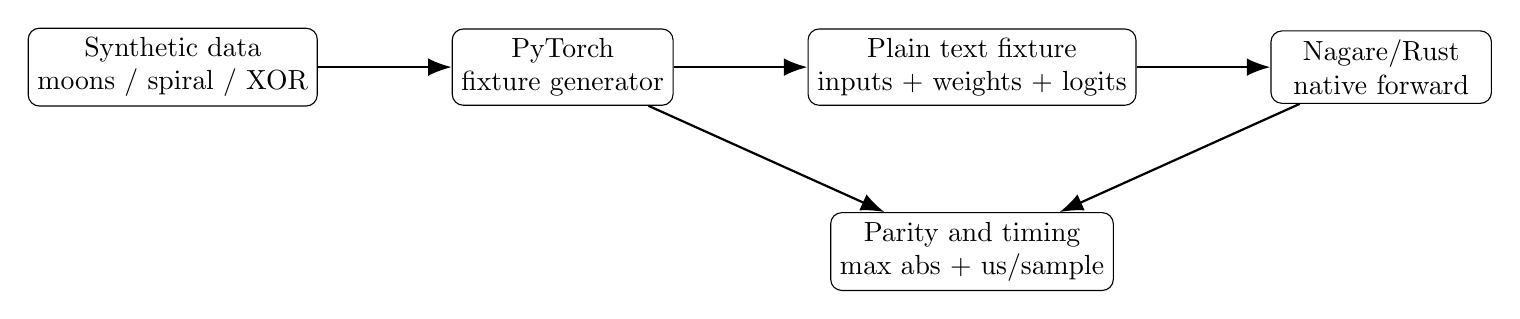
\begin{tikzpicture}[
  node distance=1.35cm and 1.7cm,
  box/.style={draw, rounded corners, align=center, minimum width=2.8cm, minimum height=0.9cm},
  small/.style={draw, rounded corners, align=center, minimum width=2.2cm, minimum height=0.75cm},
  arrow/.style={-{Latex[length=3mm]}, thick}
]
\node[box] (data) {Synthetic data\\moons / spiral / XOR};
\node[box, right=of data] (pt) {PyTorch\\fixture generator};
\node[box, right=of pt] (fixture) {Plain text fixture\\inputs + weights + logits};
\node[box, right=of fixture] (ng) {Nagare/Rust\\native forward};
\node[box, below=of fixture] (cmp) {Parity and timing\\max abs + us/sample};

\draw[arrow] (data) -- (pt);
\draw[arrow] (pt) -- (fixture);
\draw[arrow] (fixture) -- (ng);
\draw[arrow] (pt) -- (cmp);
\draw[arrow] (ng) -- (cmp);
\end{tikzpicture}
}%
\end{center}

The fixture path makes the comparison strict: PyTorch and Nagare receive the
same samples, the same weights, and the same expected logits. Accuracy here is
only a sanity check because the weights are random; the real metric is exact
forward parity and runtime.

\subsection{Native Chebyshev Deploy Classifier}

\begin{center}
\resizebox{\linewidth}{!}{%
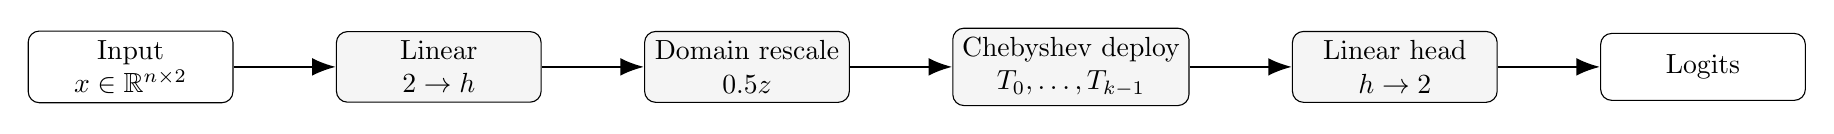
\begin{tikzpicture}[
  node distance=1.25cm and 1.3cm,
  box/.style={draw, rounded corners, align=center, minimum width=2.6cm, minimum height=0.85cm},
  op/.style={draw, rounded corners, fill=gray!8, align=center, minimum width=2.6cm, minimum height=0.85cm},
  arrow/.style={-{Latex[length=3mm]}, thick}
]
\node[box] (x) {Input\\\(x\in\mathbb{R}^{n\times2}\)};
\node[op, right=of x] (lin1) {Linear\\\(2\rightarrow h\)};
\node[op, right=of lin1] (bound) {Domain rescale\\\(0.5z\)};
\node[op, right=of bound] (cheb) {Chebyshev deploy\\\(T_0,\dots,T_{k-1}\)};
\node[op, right=of cheb] (head) {Linear head\\\(h\rightarrow2\)};
\node[box, right=of head] (logits) {Logits};

\draw[arrow] (x) -- (lin1);
\draw[arrow] (lin1) -- (bound);
\draw[arrow] (bound) -- (cheb);
\draw[arrow] (cheb) -- (head);
\draw[arrow] (head) -- (logits);
\end{tikzpicture}
}%
\end{center}

This is the architecture where Nagare is both smaller and faster. The direct
Chebyshev deploy kernel avoids CR gather, and the pre-curve adapter is a scale
into the Chebyshev domain rather than a saturating neural activation. After
removing a per-scalar temporary allocation, deploy runs in the sub-microsecond
to low-microsecond range on the measured small shapes.

\subsection{Current Entropy-Feedback Path}

\begin{center}
\resizebox{\linewidth}{!}{%
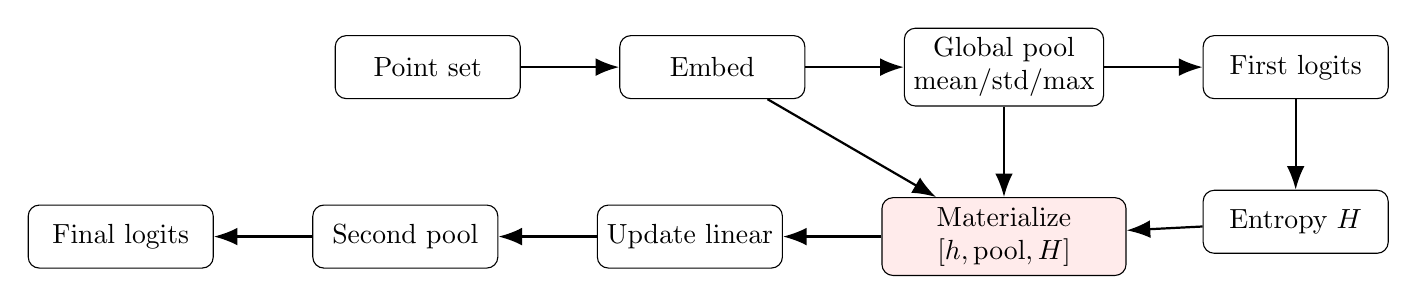
\begin{tikzpicture}[
  node distance=1.15cm and 1.25cm,
  box/.style={draw, rounded corners, align=center, minimum width=2.35cm, minimum height=0.8cm},
  bad/.style={draw, rounded corners, fill=red!8, align=center, minimum width=3.1cm, minimum height=0.9cm},
  arrow/.style={-{Latex[length=3mm]}, thick}
]
\node[box] (x) {Point set};
\node[box, right=of x] (embed) {Embed};
\node[box, right=of embed] (pool) {Global pool\\mean/std/max};
\node[box, right=of pool] (first) {First logits};
\node[box, below=of first] (ent) {Entropy \(H\)};
\node[bad, below=of pool] (mat) {Materialize\\\([h,\mathrm{pool},H]\)};
\node[box, left=of mat] (update) {Update linear};
\node[box, left=of update] (pool2) {Second pool};
\node[box, left=of pool2] (out) {Final logits};

\draw[arrow] (x) -- (embed);
\draw[arrow] (embed) -- (pool);
\draw[arrow] (pool) -- (first);
\draw[arrow] (first) -- (ent);
\draw[arrow] (pool) -- (mat);
\draw[arrow] (ent) -- (mat);
\draw[arrow] (embed) -- (mat);
\draw[arrow] (mat) -- (update);
\draw[arrow] (update) -- (pool2);
\draw[arrow] (pool2) -- (out);
\end{tikzpicture}
}%
\end{center}

This is the architecture where Nagare is smaller but currently slower. The red
node is the problem: it allocates a wide broadcast tensor and makes the native
Rust path resemble a PyTorch-style composed tensor program.

\subsection{Target Fused Entropy-Feedback Path}

\begin{center}
\resizebox{\linewidth}{!}{%
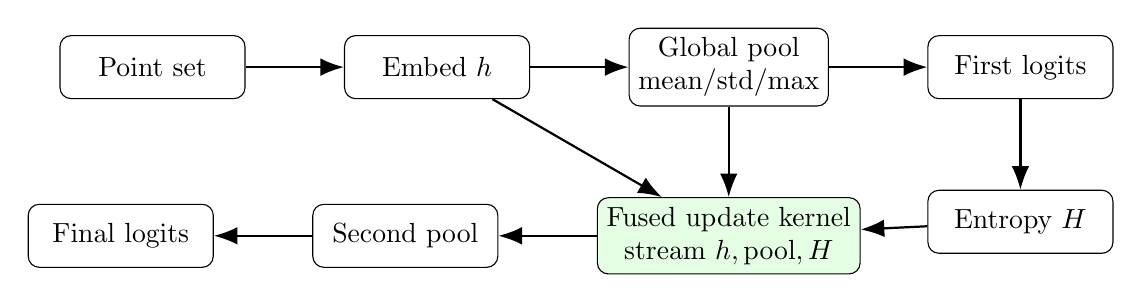
\begin{tikzpicture}[
  node distance=1.15cm and 1.25cm,
  box/.style={draw, rounded corners, align=center, minimum width=2.35cm, minimum height=0.8cm},
  good/.style={draw, rounded corners, fill=green!10, align=center, minimum width=3.1cm, minimum height=0.9cm},
  arrow/.style={-{Latex[length=3mm]}, thick}
]
\node[box] (x) {Point set};
\node[box, right=of x] (embed) {Embed \(h\)};
\node[box, right=of embed] (pool) {Global pool\\mean/std/max};
\node[box, right=of pool] (first) {First logits};
\node[box, below=of first] (ent) {Entropy \(H\)};
\node[good, below=of pool] (fused) {Fused update kernel\\stream \(h,\mathrm{pool},H\)};
\node[box, left=of fused] (pool2) {Second pool};
\node[box, left=of pool2] (out) {Final logits};

\draw[arrow] (x) -- (embed);
\draw[arrow] (embed) -- (pool);
\draw[arrow] (pool) -- (first);
\draw[arrow] (first) -- (ent);
\draw[arrow] (embed) -- (fused);
\draw[arrow] (pool) -- (fused);
\draw[arrow] (ent) -- (fused);
\draw[arrow] (fused) -- (pool2);
\draw[arrow] (pool2) -- (out);
\end{tikzpicture}
}%
\end{center}

The target kernel should compute the update linear directly from the local
embedding row, pooled context, and entropy scalar. It should not allocate
\([h,\mathrm{pool},H]\). This is the next step needed to make the
entropy-feedback architecture match the smaller-and-faster behavior observed
for Chebyshev deploy.

\section{Decision}

The result should be used as a development gate:

\begin{enumerate}
  \item Promote direct Chebyshev deploy as the small CPU inference path.
  \item Keep CR and Chebyshev-CR train mode as native training-quality operators.
  \item Implement fused entropy-feedback update before making any broader speed
        claim for the global-pool entropy model.
  \item Re-run exact PyTorch parity after the fused update kernel lands.
\end{enumerate}

\section{Evidence Trail}

\begin{itemize}
  \item \texttt{reports/2026-07-01-nagare-pytorch-synthetic-cheby-compare.md}
  \item \texttt{reports/2026-07-01-nagare-cr-cheby-small-perf.md}
  \item \texttt{reports/2026-07-01-nagare-pytorch-global-pool-entropy-parity.md}
  \item \texttt{reports/2026-07-01-nagare-smaller-faster-summary.md}
\end{itemize}

\end{document}
